\chapter{Technik}
\label{technik}

Beim Tischfussball ist das Toreschiessen das wichtigste um zu Gewinnen und daher ist das Spiel von Anfängern durch viele schnelle (Direkt-)Schüße geprägt.
Vor allem durch \textbf{Trickschüsse} heben sich erfolgreichere Spieler hervor.
Im Amateur-Bereich kommen meist Pass- und Schuss-Optionen hinzu.
Und im Profi-Bereich werden meist alle \textbf{Techniken} angewandt, vor allem um strategisch eine Partie zu gewinnen. siehe nächstes Kapitel~\ref{taktik}. 
Bei allen Spielniveaus werden verschiedene Defensivtechniken angewandt, um die Offensive des Gegners erfolgreich zu verteidigen.
All diese Techniken sind notwendig für ein \textbf{kontrolliertes Spiel} -- was der eigentlich Trick der Profis ist.

Technik ist die Grundlage eines jeden Sports. 
Das Ziel einer sauberen Technik ist das Kontrollieren des Balles mit den Spielfiguren in unterschiedlichen Spielsituationen:
\begin{itemize}
    \item in der \textbf{Offensive und bei Ballbesitz} gibt es folgende Techniken (Kapitel \ref{technik:offensive}):
        \begin{itemize}
            \item das Passen, 
            \item das Annehmen und 
            \item das Schießen des Balles
        \end{itemize}
    \item in der \textbf{Defensive  und bei Nicht-Ballbesitz} gibt es folgende Techniken (Kapitel \ref{technik:defensive}):
        \begin{itemize}
            \item das Stellungsspiel, 
            \item das Blocken und 
            \item das Fangen des Balles  
        \end{itemize}
\end{itemize}
Zunächst in Kapitel \ref{technik:haltung} wird die grundlegende Körper- und Griffhaltung beschrieben, wobei sich vor allem die Griffhaltung und Arm- und Oberkörperbewegung beim Spielen der Techniken verändern kann. 

\paragraph{Technik-Training;} 
Das Erlernen der Techniken und entprechendes Training sollte \textbf{dem Spielniveau und dem Alter angepasst} werden. 
Spielerisches Erlenen (siehe Kapitel~\ref{chap:spielformen}) ist etwa für Kinder und Jugendliche und Anfänger geeignet, regelmäßige Wettkämofe (Liga und Turniere) für Fortgeschrittene und statisches Techniktraining für ambitionierte Spieler.


%%%%%%%%%%%%%%%%%%%%%%%%%%%%%%%%%%%%%%%%%%%%%
\section{Körper- und Handhaltung}
\label{technik:haltung}

Bei \textbf{Ballsportarten} sind die Körperstellung und der Stand zum Ball eine Grundvorraussetzung zum erfolgreichen Spiel.
Bei \textbf{Schlägersportarten} sind die Handhaltung und die Arm- und Körperbeweglichkeit eine Grundvorraussetzung zur erfolgreichen Ausführung einer Spielaktion.
Diesen beiden Aspekte sind auch beim Tischfussball zu beachten:
Ein richtiger \textbf{Stand} zum Tisch beinhaltet eine eine lockere Grundbeweglichkeit von Körper und vor allem den Armen und Händen zum Bewegen der Stangen (Kapitel~\ref{technik:haltung:koerper}),
Eine richtige \textbf{Handhaltung} der Stangen umfasst das einer Spielsituation bedingtes Drehen und Schieben und Ziehen der Stangen und damit Spielen des Balles (Kapitel~\ref{technik:haltung:griffe}).
Die folgenden Kapitel geben eine grundlegende Richtlinie zur richtigen Haltung, die für jeden \textbf{individuell} anders ist. 

\begin{figure}
    \centering 
        \begin{subfigure}[b]{0.9\textwidth} 
            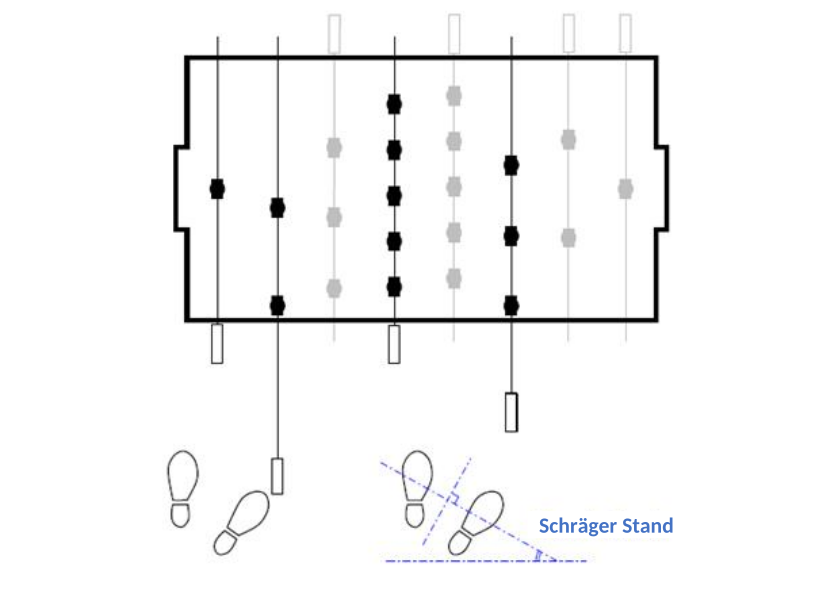
\includegraphics[width=\textwidth]{img/haltung_koerper.png} 
            \caption{Grundlegender Körperstand} 
            \label{fig:haltung:koerper} 
            \vspace{0.5cm}
        \end{subfigure} 
        \begin{subfigure}[b]{0.5\textwidth} 
            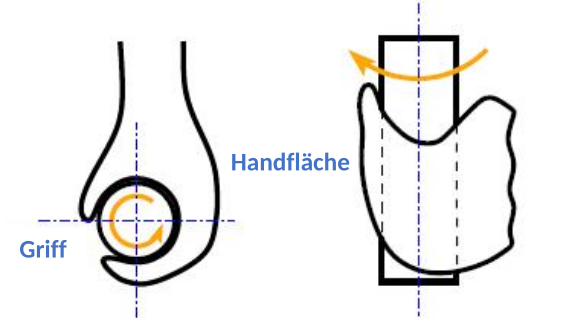
\includegraphics[width=\textwidth]{img/haltung_hand.png} 
            \caption{Grundlegende Handhaltung} 
            \label{fig:haltung:hand} 
        \end{subfigure} 
        \label{fig:haltung} 
        \caption{Die grundlegenden Haltungen [\cite{itsf_basics}]} 
\end{figure}

%%%%%%%%%%%%%%%%%%%%%%%%%%%%%%%%%%%%%%%%%%%%%
\subsection{Körperhaltung}
\label{technik:haltung:koerper}

Die Grundhaltung ist ein \textbf{schulterbreiter} Stand.
Der Abstand vom Körper zum Tisch mit einem leichten \textbf{schrägen Stand} mit Blick zum Tor (siehe Abbildung \ref{fig:haltung:koerper}) sollte so sein, dass die Stangen beweglich ganz rein- und rausgefahren und gedreht werden können.
Dabei kann der rechte Arm aus der Schulter seitlich am Körper vor und zurück bewegt werden. 

Ein \textbf{lockerer} Stand sollte die Arme für flüssige Stangenbewegungen entlasten. 
Daher sollte man sich etwa nicht auf den Griffen abstützen.
Hierbei hilft es leicht in die Knie zu gehen und das Körpergewicht leicht auf die Fussballen zu verlagern; der Oberkörper ist meist gebeugt zum Tisch, dabei sollte der Rücken einigermaßen gerade und die Schultern locker sein.

Diese Grundhaltung ist \textbf{statisch}, dass bedeutet die Füße behalten ihre Position. 
Meist wird diese statische Haltung weitestgehend bei der Ausführung eines Passes oder Schusses beibehalten. 
Positionsänderungen passieren für einen \textbf{angepassten Stand} etwa für eine bestimmte Schusstechnik (Zieher, Schieber, Abroller, Front-Pin) und Defensivtechniken (\textbf{Körpersetup}).
Und in der Einzeldisziplin muss der Spieler sich am Tisch ständig bewegen und seine Position der jeweiligen Ballposition bzw. der gewollten Stangenkontrolle anpassen.

\paragraph{Hinweis:} Um Rückenproblemen vorzubeugen, sollte neben der entspannten Körperhaltung eine Ausgleichsbewegung vor oder nach dem Tischfussballspielen gemacht werden.
Das kann eine andere Sportart sein, aber auch schon ein paar kurze Aufwärm- und Lockerungsübungen können entspannen: Hüpfen, Armkreisen, Luftklettern, usw. 

\paragraph{Lese-Tipp:} \href{http://ungeblogtkickern.blogspot.de/2016/07/korperhaltung.html}{Artikel auf Ungeblogt}

%%%%%%%%%%%%%%%%%%%%%%%%%%%%%%%%%%%%%%%%%%%%%
\subsection{Handhaltung}
\label{technik:haltung:griffe}

Bei der Handhaltung gibt es für die meisten Techniken eine Standard-Handhaltung und viele speziell angepasste Handhaltungen für bestimmte Pass-, Schuss- und Haltetechniken (\textbf{Handsetup}). 
Die Standard-Handhaltung ist eine \textbf{geschlossene}
und der Handrücken zeigt dabei nach oben (siehe Abbildung~\ref{fig:haltung:hand}).
Wird der Griff so gehalten, wenn gleichzeitig die Figuren mit den Füßen nach unten stehen, kann die Stange durch Bewegen des Handgelenks so gedreht werden, dass die Füße der Figuren die \textbf{volle Drehbereich abfahren} (siehe Abbildung~\ref{fig:figurdrehen}):
\begin{itemize}
    \item von ganz hinten, um einen \textbf{Ball hinter der Stange} zu spielen (Hinten Klemmen, Back-Pin, Brush/Drücker, Druckpunkt, Fangen, siehe Kapitel \ref{}), über
    \item gerade Figuren-Position für Tic-Tac (Kapitel \ref{}) die volle Abdeckung (Kapitel \ref{}) bis 
    \item ganz vorne, um einen \textbf{Ball vor der Stange} zu spielen (Vorne Klemmen, Front-Pin, Fangen, siehe Kapitel \ref{}).
\end{itemize}

\begin{figure}
    \centering 
        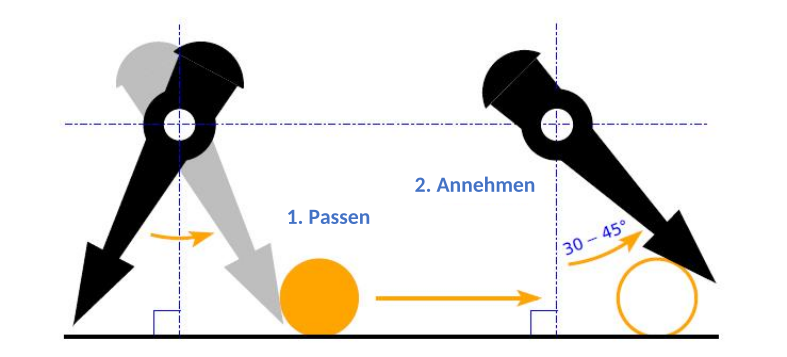
\includegraphics[width=0.7\textwidth]{img/haltung_figur.png} 
        \caption{Drehung der Stange: Verschiedene Figurpositionen, hinter der Stange (links), rechts vor der Stange (rechts) [\cite{itsf_basics}]} 
        \label{fig:haltung:figur} 
\end{figure}

Der Griff wird je nach Technik \textbf{unterschiedlich stark festgehalten} oder mit \textbf{verschiedenen Drehgeschwindigkeiten} bewegt.
Grundsätzlich lässt eine lockere Handhaltung die Stange in den Lagern frei und damit letztendlich schnell bewegen.
Das gilt für Seitwärts-Bewegungen der Stange und für Drehbewegungen der Stange.

Je nach Körperhaltung und Position, ist der \textbf{Unterarm unterschiedlich geneigt} und damit die Achse des Handgelenks unterschiedlich zur Drehachse der Stange.
Hier gibt es Anpassungen je nach Technik (Zieher, Schieber, Linke-Hand-Pass, Defensiv-Stellungen) oder nach indivueller Haltung.
Dies ist auch abhängig von der Körpergröße. 
Für Kinder und Jugendliche gibt es daher Podeste die den Stand um bis zu 20 cm erhöhen können (siehe auch \ref{}).


Eine erste abweichende Griffhaltung ist der \textbf{Fingergriff}: Hierbei halten die Fingerspitzen das Griff Ende, der Unterarm ist fast waagrecht, und die Stange kann aus dem Unterarm schnell gedreht werden.
Für die Schusstechniken Abroller/Front-Pin und Jet gibt es mit \textbf{Affenhand und Handgelenkshaltung} komplett andere Grundhaltungen des Griffs, siehe Kapitel~\ref{} bzw. \ref{}.


%%%%%%%%%%%%%%%%%%%%%%%%%%%%%%%%%%%%%%%%%%%%%
%%%%%%%%%%%%%%%%%%%%%%%%%%%%%%%%%%%%%%%%%%%%%
\section{Offensive: Passen, Annehmen, Schiessen}
\label{technik:offensive}

Beim Tischfussball ist die \gls{offensive} bei Ballbesitz möglich.
Dabei können die Figuren durch Bewegen der Stange nur im jeweiligen Bereich den Ball erreichen und spielen (vergleiche Abbildung~\ref{fig:tischbereiche}).
Ballkontrolle oder Ballgefühl beinhalten das Passen, das Annehmen und das Schiessen des Balles.

%%%%%%%%%%%%%%%%%%%%%%%%%%%%%%%%%%%%%%%%%%%%%
\subsection{Ballführung (auf einer Stange)} 
\label{technik:offensive:eine}

Bei der Ballführung auf einer Stange wird der Ball entlang der Stange von Puppe zur Puppe und gegebenfalls Bande gespielt. 
Die Ballführung ist die Grundlage und Vorbereitung für jeden Pass und Schuss.
Hierbei gibt es folgende unterschiedlichen Ballverläufe mit unterschiedlicher Technik:
\begin{itemize}
    \item unter der Stange durch Tic-Tac
    \item Hinten oder Vorne geklemmt durch die Pin-Technik
    \item Vorne-Hinten geklemmt im Wechsel durch die Pin-Technik
\end{itemize}

\subsubsection{Tic-Tac}
"Tic-Tac" nennt man das direkte Hin- und Herspielen zwischen Figuren, zwischen Figur und Bande, zwischen der nächsten Figur durch zwischenzeitliches Hochklappen. 
\begin{itemize}
    \item \textbf{Körper- und Handsetup:} Standard 
    \item \textbf{Pasen:} Der Ball wird mit gerade Figur seitlich angestossen, geschoben oder gezogen ("Tic"\ oder "Tac").
    \item \textbf{Annahme:} Der Ball wird durch Nachführen der Figur gestoppt oder direkt gespielt.
    \item \textbf{Korrigieren}: Durch Drehen der Figur kann der Ball unter der Stange gehalten werden: Durch die Fläche kann der Ball Richtung Stange geleitet werden oder durch schräges Passen durch Drehung der Figur.  
    \item \textbf{Übungen und Variationen}:
        \begin{itemize}
            \item zwischen zwei Figuren, z.B. auf der 2er-Stange zwischen der 1. und der 2. Puppe.
            \item zwischen einer Figur und einer Bande
            \item zwischen der übernächsten Figur durch zwischenzeitliches Hochklappen der nächsten Figur, z.B. auf der 3er-Stange zwischen der 1. und der 2. Puppe oder der 2. und der 3.Puppe oder mit der 1. und 3. Puppe, oder auf der 5er-Stange zwischen der zwei benachbarten Puppen oder mit zwei Puppen und dabei eine Puppe auslassen.
            \item auf der 2er-, 5er- oder 3er-Stange jeweils mit Rechts oder Links, z.B. beim Spiel ,,Alle 11 Figuren'': Bei hochgeklappten gegnerischen Figuren, passt der Spieler sich von der Torwart-, über die 2er- und 5er- bis zu 3er-Stange durch Tic-Tac. 
            \item Anlaufen lassen und sanft Abstoppen. Diese Fertigkeit ist vor allem für eine sichere Zieher- oder Schieber-Auflage winchtig.
        \end{itemize}
\end{itemize}


\subsubsection{Pin-Technik}
Die Pin-Technik ist die Ballführung in dem der Ball auf seinem Scheitelpunkt (Ausgangspostion) durch die Fussspitze der schrägen Figur geführt und gespielt wird.
\begin{itemize}
    \item \textbf{Körper- und Handsetup:} Standard 
    \item \textbf{Pasen:} Der Ball wird durch seitliches Bewegen mit der Pin-Technik zur nächsten Figur. Durch leichten Druck auf den Ball läuft der Ball parallel zur Stange; durch erhöhten Druck unter die Stange läuft der Ball unter die Stange
    \item \textbf{Annahme:} Der Ball wird durch die Pin-Technik gestoppt und der Ball eingeklemmt.
    \item \textbf{Korrigieren}: Wurde der Ball nicht ganz auf dem Scheitelpunkt gefangen, kann der Ball durch leichtes Klopfen auf den Ball in die Pin-Ausgangsposition gebracht werden.
    \item \textbf{Übungen und Variationen}:
        \begin{itemize}
            \item zwischen zwei Figuren, z.B. auf der 3er-Stange zwischen den Puppen
            \item zwischen der übernächsten Figur durch zwischenzeitliches Hochklappen der nächsten Figur, z.B. auf der 5er-Stange zwischen den Puppen
            \item vorne und hinten geklemmt auf einer Figur
            \item vorne und hinten geklemmt mit mehreren Figuren, z.B. auf der 3er-Reihe das "V"\  in beide Richtungen, auf der 5er-Stange das "W"\ in beide Richtungen oder auf der 2er-Reihe das ,,I'' in beide Richtungen und als Variation mit Einbindung des Torwarts
        \end{itemize}
\end{itemize}

%%%%%%%%%%%%%%%%%%%%%%%%%%%%%%%%%%%%%%%%%%%%%
\subsection{Passen (zwischen zwei Stangen)}
\label{technik:offensive:zwei}

Passen ist Spielen zwischen den eigenen Stangen, das genaue Spielen des Balles und das Annahmen und Stoppen des Balles.
Es gibt folgende üblichen \textbf{Pass-Szenarien oder offensive Spielzüge}:
\begin{itemize}
    \item Als Verteidiger zwischen Torwart- und 2er-Stange
    \item Als Verteidiger vom dem Verteidigungsbereich auf die 3er-Stange des Stürmers
    \item Als Stürmer von der 5er- auf die 3er-Stange
    \item Im Einzel von der 2er-Stange (linke Hand) auf die 5er-Stange oder auf die 3er-Stange
\end{itemize}

Beim Passen gibt es \textbf{verschiedene Passtechniken}:
\begin{itemize}
    \item Gerade oder Drücker (gerade): Der Ball liegt unter der Stange und wird durch Ausholen und gerade Drehbewegung nach vorne gepasst. 
        Liegt der Ball weit unter der Stange, kann der Ball, indem die Figur direkt am Ball startet, nach vorne gedrückt werden. 
        Beim sogenannten \textbf{Druckpunkt} ist wenig Kraftaufwand notwendig, um den Ball stark zu beschleunigen.
    \item Brush (schräg): Beim Brush oder dem Wischen liegt der Ball auch unter der Stange nahe am Druckpunkt und wird durch seitliche Stangenbewegung und gleichzeitige Drehbewegung schräg nach vorne gewischt.  
        Durch Variation dieser beiden Bewegungen kann der Ball unterschiedlich schräg und schnell gepasst werden.
    \item Kantenpass (schräg): Hier liegt der Ball im Bereich unter der Stange und wird durch Treffen der Figur mit der Kante schräg nach vorne gespielt.
\end{itemize}
Zum Schräg-Passen und Schiessen gibt es einen \href{http://ungeblogtkickern.blogspot.de/2015/09/schrag-schieen.html}{Artikel auf Ungeblogt}.
Eine Spass-Technik ist der sogenannter Quetscher, hierbei ist der Ball mit der Pin-Technik hinten geklemmt und durch seitliches Bewegen und gleichzeitig viel Dreh-Druck unter die Stange wird der Bal seitlich herausgequetscht.

Bei der \textbf{Ballahname} sollte die Figur grundsätzlich nach vorne gestellt sein und zum Stoppen des Balls ein leichtes Dach mit der Figur gebildet werden. 
Die Neigung der Figur hängt von der Stärke der Griffhaltung und einer mit dem Ball mitdrehender Bewegung ab: 
Ist der Fuss weit vorne kann durch eine starre Figur der Ball direkt eingeklemmt auf der Stange bleiben.
Ein moderater Ball kann durch lockere Griffhaltung und leichtes Mitdrehen der Stange der Ball abgebremst und zum Stoppen gebracht werden.

In Kapitel \ref{} wird mit den Pass-Systemen die Strategie und Taktik erklärt, hier folgen verschiedne \textbf{Technik-Übungen und Trainingsspiele}: 
\begin{itemize}
    \item Für den Verteidiger: Zwischen Torwart und einer 2er-Figur gerade hin- und herspielen. Als Variation Ballmitnahme und zwischenzeitliches Stoppen, verschiedene Geschwindigkeiten, oder mit seitlichen Bewegen und Abfahren des verlängerte Torbereichs (vergleiche Hilfslinien auf Tischgrafik).  
Im Abwehrbereich werden üblicherweise ausnahmsweise auch Pässe nach hinten gemacht: Mit der 2er-Stange kann der Ball an die Torbande gespielt werden und mit der gleiche Puppe gefangen werden.
    \item Für den Stürmer: Zwischen der 5er- und 3er-Stange hin- und her spielen. Durch seitliches Spielen alle Puppen durchwechseln.
    \item Für das Doppel: Verteidiger passt auf die 3er-Stange. Als Variation verschiedene schräge und starke Pässe.  
    \item Für das Einzel: Mit der linke Hand von der 2er-Stange auf die 5er- oder 3er-Stange mit der rechten Hand.
\end{itemize}




%%%%%%%%%%%%%%%%%%%%%%%%%%%%%%%%%%%%%%%%%%%%%
\subsection{Torschüsse}
\label{technik:offensive:torschuesse}

\begin{itemize}
\item Schussprinzipien: Schneller als der Gegner, Seitwärtsbewegung und Schussbewegung. Für Fortgeschrittene: Geschwindigkeit, Präzision, Konstanz, Abrufbarkeit
\item Schusstechniken: Schieber/Zieher, \href{http://ungeblogtkickern.blogspot.de/2014/07/schritt-fur-schritt-pin-schieen.html}{Abroller/Pin} oder Jet.
\item Von der 3er-Stange oder der 2er-Reihe.
\item Trickschüsse
\end{itemize}





%%%%%%%%%%%%%%%%%%%%%%%%%%%%%%%%%%%%%%%%%%%%%
%%%%%%%%%%%%%%%%%%%%%%%%%%%%%%%%%%%%%%%%%%%%%
\section{Defensive: Stellen, Blocken, Fangen}
\label{technik:defensive}

\begin{itemize}
\item Defensiv-Prinzip: mit den Figuren die direkten Ballwege zum Tor blockieren (Seitwärtsbewegung)  
\item Klapprichtung der Figuren und Abstand der Figuren (Drehbewegung)
\item Bälle blocken, fangen, annehmen 
\end{itemize}
Daraus folgen grundlegende sogenannte Stellungsspiele.


\subsection{Ballbesitz des Gegners im Abwehrbereich}
\label{technik:defensive:gegnerabwehr}

\begin{itemize}
\item Deckung als Stürmer
\item Deckung als Torwart: (statisch) im kurzen/langen Eck
\item Deckung im Doppel
\item Deckung im Einzel
\end{itemize}


\subsection{Ballbesitz des Gegners im Mittelfeld (5er-Reihe)}
\label{technik:defensive:gegnermittelfeld}

\begin{itemize}
\item Deckung als Stürmer (5er-Reihe): Pass verhindern, kleinster Fahrbereich, an die Bande fahren
\item Deckung als Torwart: Torschüße, direkter Ballweg
\end{itemize}


\subsection{Ballbesitz des Gegners im Sturm (3er-Reihe)}
\label{technik:defensive:gegnersturm}

\begin{itemize}
\item Deckung als Torwart: Reaktion, fahren, shaken, Wechseln
\end{itemize}

